\documentclass[10pt]{standalone}
\usepackage[utf8]{inputenc}
\usepackage{pgf,tikz }
%\pgfplotsset{compat=1.15}
\usepackage{mathrsfs}
\usetikzlibrary{arrows}
\pagestyle{empty}
\begin{document}

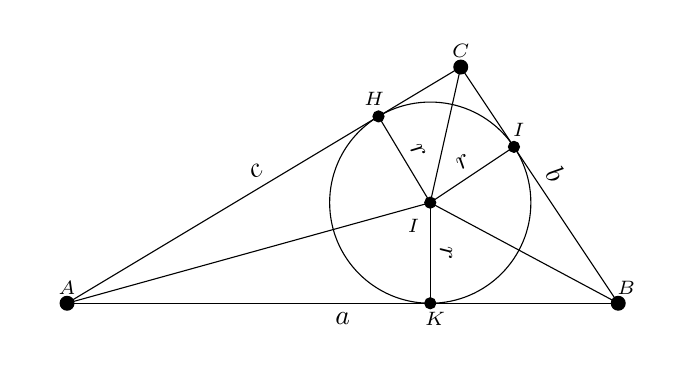
\begin{tikzpicture}[line cap=round,line join=round,>=triangle 45,x=1.0cm,y=1.0cm]

\clip(-0.5,-0.5) rectangle (7.5,3.5);
\draw  (0.,0.)-- (7.,0.)node[pos=0.5, sloped,below] {$a$};
\draw  (7.,0.)-- (5.,3.)node[pos=0.5, sloped,above] {$b$};
\draw  (5.,3.)-- (0.,0.)node[pos=0.5, sloped,above] {$c$};
\draw  (4.612700309690656,1.277644020896985) circle (1.2776440208969848cm);
\draw  (4.612700309690656,1.2776440208969848)-- (3.9553578839917987,2.3732147303950795)node[pos=0.5, sloped,above] {$r$};
\draw  (4.612700309690656,1.2776440208969848)--(5.675764393336978,1.9863534099945332)node[pos=0.5, sloped,above] {$r$};
\draw  (4.612700309690656,1.2776440208969848)-- (4.612700309690656,0.)node[pos=0.5, sloped,above] {$r$};
\draw  (4.612700309690656,1.2776440208969848)-- (0.,0.);
\draw  (4.612700309690656,1.2776440208969848)-- (7.,0.);
\draw  (4.612700309690656,1.2776440208969848)-- (5.,3.);
\begin{scriptsize}
\draw [fill=black] (0.,0.) circle (2.5pt);
\draw (0.0,0.2) node {$A$};
\draw [fill=black] (7.,0.) circle (2.5pt);
\draw (7.1,0.2) node {$B$};
\draw [fill=black] (5.,3.) circle (2.5pt);
\draw (5.0,3.2) node {$C$};

\draw [fill=black] (4.612700309690656,1.2776440208969848) circle (2.0pt);
\draw (4.4,0.98) node {$I$};
\draw [fill=black] (3.9553578839917987,2.3732147303950795) circle (2.0pt);
\draw (3.9,2.6) node {$H$};
\draw [fill=black] (5.675764393336978,1.9863534099945332) circle (2.0pt);
\draw (5.736569639044845,2.2) node {$I$};
\draw [fill=black] (4.612700309690656,0.) circle (2.0pt);
\draw (4.67489768844735,-0.2) node {$K$};

\end{scriptsize}

\end{tikzpicture}
\end{document}